\documentclass[review]{elsarticle}

\usepackage{lineno,hyperref}
\modulolinenumbers[5]

\journal{Biomedical Signal Processing and Control}

%%%%%%%%%%%%%%%%%%%%%%%
%% Elsevier bibliography styles
%%%%%%%%%%%%%%%%%%%%%%%
%% To change the style, put a % in front of the second line of the current style and
%% remove the % from the second line of the style you would like to use.
%%%%%%%%%%%%%%%%%%%%%%%

%% Numbered
%\bibliographystyle{model1-num-names}

%% Numbered without titles
%\bibliographystyle{model1a-num-names}

%% Harvard
%\bibliographystyle{model2-names.bst}\biboptions{authoryear}

%% Vancouver numbered
%\usepackage{numcompress}\bibliographystyle{model3-num-names}

%% Vancouver name/year
%\usepackage{numcompress}\bibliographystyle{model4-names}\biboptions{authoryear}

%% APA style
%\bibliographystyle{model5-names}\biboptions{authoryear}

%% AMA style
%\usepackage{numcompress}\bibliographystyle{model6-num-names}

\usepackage{amsmath}
\usepackage{amsfonts}
\usepackage{amssymb}
\usepackage{booktabs}

\usepackage{subfigure}

%% `Elsevier LaTeX' style
\bibliographystyle{elsarticle-num}
%%%%%%%%%%%%%%%%%%%%%%%

\begin{document}

\begin{frontmatter}

\title{Capturing Waveforms in Polysomnography}

%% Group authors per affiliation:
\author{Giulia Carbonari}
\author{Juliana Gambini}
\author{Juan Miguel Santos}
\author{Cecilia Forcato}
\author{Rodrigo Ramele\corref{mycorrespondingauthor}}
\address{Instituto Tecnológico de Buenos Aires}

%% or include affiliations in footnotes:
%\author[mymainaddress,mysecondaryaddress]{Elsevier Inc}
%\ead[url]{www.elsevier.com}

%\author[mysecondaryaddress]{Global Customer Service\corref{mycorrespondingauthor}}
\cortext[mycorrespondingauthor]{Corresponding author}
\ead{rramele@itba.edu.ar}

%\address[mymainaddress]{1600 John F Kennedy Boulevard, Philadelphia}
%\address[mysecondaryaddress]{360 Park Avenue South, New York}

\begin{abstract}
%\textbf{Background and Objective} \\
%\textbf{Methods} \\
%\textbf{Results} \\
%\textbf{Conclusion} \\
In this work, we propose a method to analyze and classify the detection of Slow Waves (SW) that are based on the extraction of descriptors of visually relevant characteristics from images of the signal plots. This procedure has the advantage that the characteristics used for classification are visually relevant and meaningful to a human observer. The characterization of these waves is essential because they play a major role in memory formation as well as in cleansing the brain of aberrant proteins, such as the precursors of Alzheimer's disease. A registered sleep technologist (RST) can identify an SW by visually observing its shape.  However, this procedure is time-consuming and the agreement rate between different experts is often very low. Considering that sleep studies are typically several hours long, manual SW detection can be very slow, and human error can occur due to examiner fatigue. For this reason, it is of great interest the automatic detection of SW, minimizing the error and the classification time.  Results on an annotated public dataset of Polysomnography (PSG) shows that the visual characterization of SW can be effectively mapped into a feature descriptor and that several classifiers used in EEG research are able to classify the signals with an accuracy similar to a visual observer.
\end{abstract}

\begin{keyword}
SIFT, EEG, waveform, NREM, Sleep, PSG
%\MSC[2010] 00-01\sep  99-00
\end{keyword}

\end{frontmatter}

\linenumbers

\section{Introduction}

A regular practice in image processing is to analyze images as bidimensional signals.  As a one-dimensional signal can be understood as a dependent quantity that varies in time,  a black-and-white image can be interpreted as having quantity values that vary for two independent variables, height and width. The method proposed in this work entails a different approach, where the opposite is proposed and one-dimensional signals are studied by how they are represented on images, how they look on an image plot.  This is specifically tailored for processing Electroencephalographic 
(EEG) signals, and can be used to analyze them based on the shape of their waveforms, graphoelements that conceive cognitive meaning or are of clinical relevance.  This provides a quantitative mapping of EEG components which at the same time convey meaning to the practitioners clinician, physician or registered sleep technologist (RST) who are studying these signals, and who traditionally analyze them visually by studying their waveforms~\cite{Cole2017,Rodenbeck2006,Schomer2010}.

This work expands the method previously published in ~\citep{Ramele2016, Ramele2018, Ramele2019}.  It establishes its modelling and extends its usage to the study of polysomnographic signals, particularly slow-wave sleep signals which are particularly suitable to be analyzed in this way.

Sleep Research is devoted to understanding the inner workings of the brain during sleep and its strong connection with memory formation.  Sleep is defined as a natural and reversible state of reduced responsiveness to external stimuli and relative inactivity, accompanied by a loss of consciousness. Sleep occurs in regular intervals and is homeostatically regulated and in mammals consists of two core sleep stages: non-rapid-eye-movement (NREM) and REM sleep, which alternate in a cyclic manner~\cite{RB,AASM}. During human NREM, the EEG shows predominant slow-wave activity, which is defined by the $0.5$ to $4.0$ Hz frequency bands and includes the $<1$ Hz slow oscillations with a peak frequency of $0.8$ Hz.  Slow oscillations comprise alterations between periods of neuronal membrane depolarization accompanied by sustained firing (up-states) and periods of membrane hyperpolarization associated with neuronal silence (down-state). In the scalp EEG, the negative peak of the slow oscillation coincides with the beginning of the down-to-up state transition, whereas the depolarizing phase of sustained firing correlates with the positive EEG deflection \cite{RB, AASM}.
The characterization of these waves is essential because they play a major role in memory formation as well as in the brain cleansing of aberrant proteins, such as the precursors of Alzheimer's disease \cite{RB, AASM}.
%Sleep Research has been studied in this way by performing Polysomnographic recordings (PSG) [22,23]. The different sleep stages are evaluated by visually marking waveforms or graphoelements in long-running electroencephalographic recordings, looking for patterns based on standardized guidelines [24]. Visual characterization includes the identification or classification of certain waveform components based on a subjective characterization (e.g., positive or negative peak polarity) or the location within the strip. It is regular to establish an amplitude difference between different waveforms from which a relation between them is reckoned and a structured index is created (e.g., sleep K-Complex is well characterized based on rates between positive vs negative amplitude) [25]. Other relevant EEG patterns for sleep stage scoring are alpha, theta, and delta waves, sleep spindles, polysplindles, vertex sharp waves (VSW), and sawtooth waves (REM Sleep).

% .  Automatic Sleep Stage Scoring Research .  

%El principal problema que veo es que la intro está basada en solucionar el scoring manual, que no se resuelve con la identificación de las ondas lentas. Si lo que se quiere solucionar es algo de ondas lentas como un evento particular (u oscilación) hay que poner esto en contexto.En ese caso se puede poner que las ondas lentas estas implicadas tanto en los procesos de formación de memorias como en la limpieza del cerebro de proteinas aberrantes como la beta amiloide, precursora de la enfermedad de alzheimer (rasch born, 2013, y el último de HOng-Viet go de sciende de alzheimer,  cirelli y tononi 2014). y ahi decir como que resulta fundamental la identificación de estas ondas 

    The traditional approach to glimpse what is happening inside the brain while sleeping has been the Polysomnography (PSG), which is mainly based on Electroencephalography, Electromyography (EMG) and Electrooculography (EOG)~\cite{Yan2019}.  Sleep research studies rely heavily on EEG graphoelements~\cite{Boostani2017} like K-Complexes and Slow Oscillations.  Particularly, Slow Waves (SW) are signal components known to be involved in memory formation processes as well as are understood to be relevant in cleaning beta-amyloid protein which is a precursor of Alzheimer's disease~\cite{Ngo2020}.  These component's identification is performed by visually marking waveforms in long-running PSG, looking for patterns based on standardized guidelines~\cite{Rodenbeck2006,RK,AASM}.   This visual characterization entails an expert's subjective decision.
   

This makes PSG signal analysis particular relevant for this methodology because it can be used to derive a metric that can describe quantitatively the similarities between signal shape components.  Sleep research requires long hours of visual inspection, hence, it will be greatly aided by automation tools that at the same time identify the signal structure in the same way as those experts who traditionally analyze these signals.

%In this study we provide the general layout of the model (section I), present a description of ... (section II) and we finally analyzed a database ... 

Here, we first provide the general layout of the model, detailed in section~\ref{materials} which presents the details of the feature extraction procedure which is implemented in an accompanying software.  For the experiment section, we analyzed a database of Sleep Research to identify Slow Waves based on their waveform structure.  In the section~\ref{results}, results are expounded and conclusions and future research directions are outlined in the last section~\ref{conclusions}.

% This can be used to obtain descriptors from images and that can be integrated into other projects to perform this analysis.  

\section{Materials and Methods}
\label{materials}
\subsection{Converting 1D signals to Images: Plotting}

An EEG signal can be considered as a multichannel time point sequence.  This sequence is obtained by a digitalization process, at a certain sampling frequency $F_s$ which depends on the electrophysiological device \cite{Jackson2014}.  The original EEG stream can be divided into segments or epochs $\tilde{x}(n,c) $ of fixed length and zero media.  These segments are extracted to be further analyzed to determine the presence or not of signal markers that are particularly relevant to EEG signal processing or sleep research.

Since a century ago, the study of these signals involved the creation of a representation in the form of a signal plot~\cite{Jestico1977}.  Plotting entails a digitalization process as well and produces a binary image per EEG channel with the trace representing the time-varying signal. 

This binary image $\mathcal{I}^{(c)}$ can be constructed based on Equation~\ref{eq:plot},

\begin{equation}
\mathcal{I}^{(c)}(z_1,z_2) = \left\{ \begin{array}{rl}
255 & \text{if} \   z_1 = \gamma_{t} \  n \quad \text{and}  \quad z_2 = \left\lfloor \gamma \; \tilde{x}(n,c) \right\rceil + z(c) \\
0   & \mbox{otherwise}
\end{array}\right.
\label{eq:plot}
\end{equation}

\noindent  where  $1 \leq c \leq C$ and $1 \leq n \leq N$, with $C$ as the number of available channels and $N$ as the length of each segment.  The coordinate $z_1$ is on the horizontal axis of the image and $z_2$ is the vertical coordinate, increasing from top to bottom, so the $(0,0)$ position is on the upper-left corner of the image.  The amplitude scale factor $\gamma$ and time scale factor $\gamma_{t}$ are used to determine the image size and at the same time the image resolution. In order to complete the trace of the signal plot, the isolated points produced by Equation~\ref{eq:plot} are connected using the Bresenham~\cite{Bresenham1965} algorithm, which performs a linear discrete interpolation between the pixels.  This scheme produces a black-and-white plot of the signal with $255$ being white and $0$ black.  There is one image per channel per segment. 

Finally, the value $z(c)$ corresponds to the position on the image where the signal is zero, the zero-level, and it is calculated as

\begin{align*}
z(c) =\Big | \left \lfloor{ \min_{n} \tilde{x}(n,c) }\right \rfloor \Big |.
\label{eq:zerolevel}
\end{align*}

This reveals that the plot of the signal is upside down on the image, where the amplitude is positive increasing to the bottom of the image, which by the way, is a regular procedure to plot signals in neuroscience~\cite{Schomer2010}.

%\noindent with $255$ being white and representing the signal's voltage in relation to the zero-level $z(c)$, and $0$ for black which is the background contrast. This scheme produces a black-and-white plot of the signal.  Pixel arguments $ (z_1,z_2) \in \mathbb{N} \times \mathbb{N}$ iterate over the width $Wx$ and height $Hy$  of the image plot with $1 \leq n \leq N$ and $1 \leq c \leq C$.  There is one image per channel.  The parameters $\gamma$ and $\gamma_t$ are the amplitude and time scaling factors.  They are used to determine the image size and at the same time the image resolution.


%\paragraph{A Digitalization Procedure} 

%\paragraph{Resolution and Precision} 


\subsection{The Scale Invariant Feature Transform Method}
\label{SIFT}

%Ijima 62
%Otsu 81
%Witkin 83
%Koenderink 84
%Lindeberg 94
%Viergever 97
%Lowe 04
%Holmstron 13

Recognizing structures from visual observation pertain to two different problems at the same time.  The first is to identify which areas of the visual scene are conveying the higher amount of information.  In a sense, what are the salient features of an image that are important to emphasize and that help to characterize what is being seen.   The second problem is precisely to give some meaning to these particular regions, to understand when they are similar to each other, or when they are different.

The first problem, the detection, found inspiration in the studies performed by~ \citep{Marr1979} on how human stereo vision works.  The work \citep{Iijima1962,Witkin1983} emphasized the importance of \textit{scale}, and that signal features that are resilient to scaling and smoothing transformations are key elements that convey important information.  These results pave the way to the development of the classical scale space methodology~\cite{Koenderink1984,Weickert1999,Lindeberg1990,Lindeberg1994,ter1997scale,Jansson2020}.

On the other hand, the seminal work of~\citep{HUBEL1965}, expanded with the work of~\cite{Edelman1997} on how the visual cortex of cats sense shapes based on the orientation of objects that were being displayed to them, pointed out towards a way to describe visual features based on how they are oriented on the visual scene.  This was further elaborated in the Theory of Receptive Fields \cite{Linde2012,Lindeberg2013}.

The Scale Invariant Feature Transform (SIFT) method was proposed by \citep{Lowe2004} and it is the confluence of these two ideas.  The SIFT Detector is the procedure to identify relevant areas of an image, based on the detection of certain regions that are obtained after applying several changes in scale and successive Gaussian filters to smooth the images~\cite{Rey-Otero2014,Szeliski2010}.  Given an image, the SIFT Detector provides a set of candidates keypoints, locations on the image with relevant features in different scales.   On the other hand, the SIFT Descriptor is the procedure to describe and characterize the regions around each keypoint, called patches, by creating a histogram of gradient orientations.  This histogram is summarized in a feature vector which effectively represents the structure of the information contained within the patch.   

%was the inspiration to the development of an algorithm to identify and decode salient local information from image regions.  

\subsection{Waveform Extraction Procedure}

The method proposed here is grounded on an extension and modification of the SIFT Descriptor.  The procedure to capture the waveform of the signal using this method is thus summarized in three steps:

\begin{enumerate}
\item Keypoints $\mathbf{kp}$ are located on an image of a signal plot.
\item A region of an image, a patch, is established using keypoints as centers.  Each patch has a horizontal $St$ and vertical scale $Sv$, which determines the size in pixels $\mathbf{S}_x$ and $\mathbf{S}_y$,  along the horizontal and vertical axis respectively. 
\item From each patch, a descriptor $\mathbf{d}$ is derived which is used as a representation of the graphical information contained within the patch.
\end{enumerate}

The keypoint $\mathbf{kp}$ represent the center location of the patch and is placed on a pixel $(x_{kp}, y_{kp})$ over the image plot. A local image patch of size $\mathbf{S}_x \times \mathbf{S}_y$ pixels is constructed around the keypoint and it is divided in $16$ blocks $B_{i,j}$. It is arranged in a $4 \times 4$ grid and the pixel $\mathbf{kp}$ is the patch center.  Figure~\ref{fig:sampledescriptor}(a) shows a plot of a signal, a keypoint at the center and the surrounding patch in green.

\begin{figure}[h!]
\centering
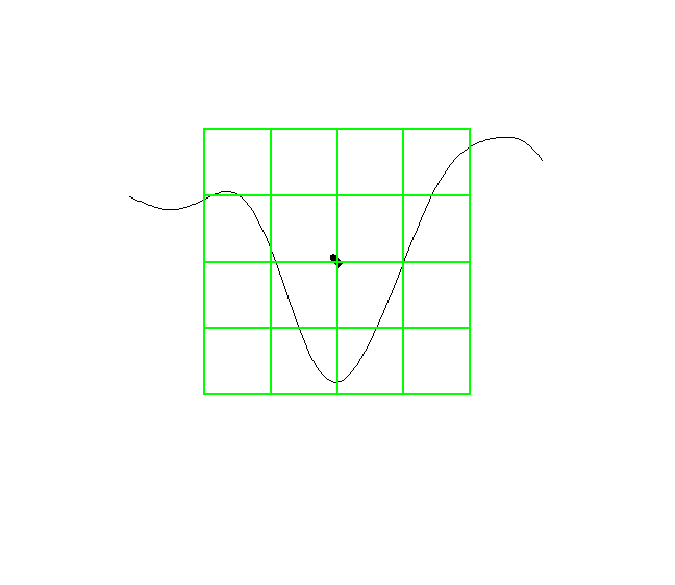
\includegraphics[width=5cm]{images/sws.eps}
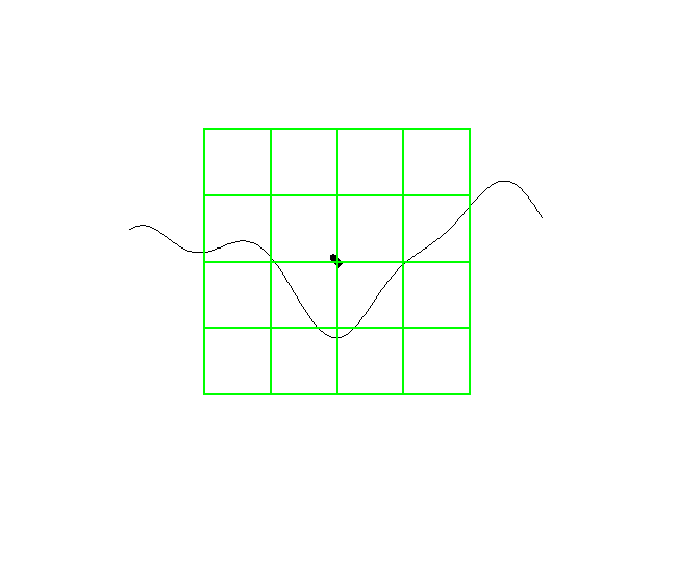
\includegraphics[width=5cm]{images/sws2.eps}
\caption[Descriptor]{Two Slow Waves (SW) are shown, with the superimposed 4x4 patch in green and the patch center as a black dot.  The Slow Waves shown here have their positive peaks upwards.}
\label{fig:sampledescriptor}
\end{figure}

Pixel intensity gradients can be obtained from an image by applying the Sobel filter~\cite{Szeliski2010} and using finite differences to obtain pixel differences on both the $x$ and $y$ direction.  Composing them as vectors, oriented gradients on each pixel can be calculated.  Figure~\ref{fig:grads} shows a vector field of oriented gradients over a region of the SW shown on the Figure~\ref{fig:sampledescriptor}.

\begin{figure}[h!]
\centering
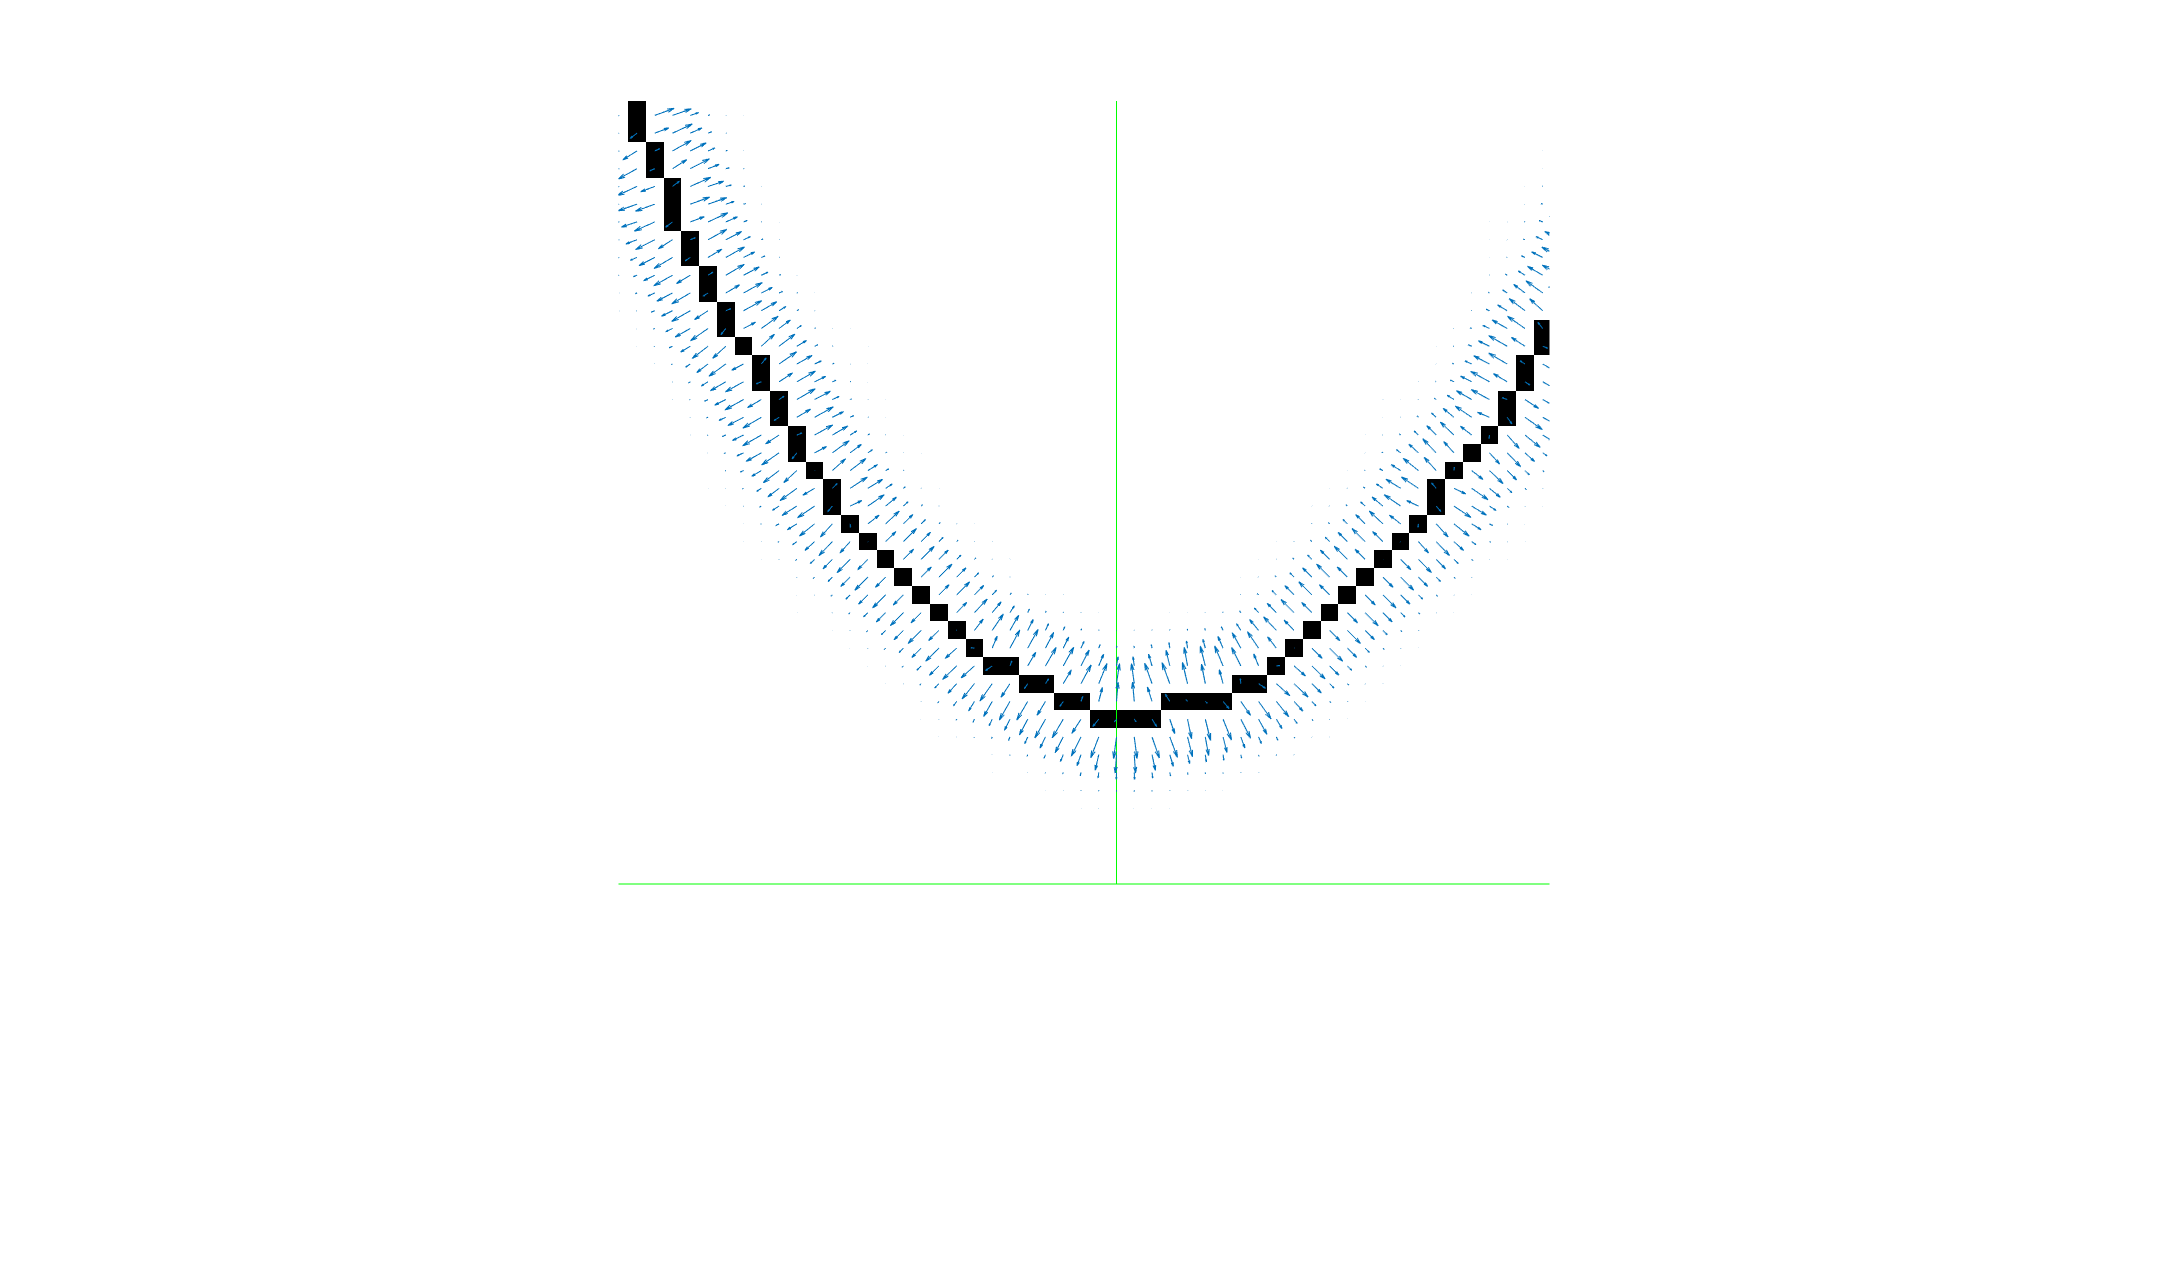
\includegraphics[width=10cm]{images/swsgrads3.eps}
\caption[Gradients]{A vector field of oriented gradients around the minimum peak of the Slow Wave shown on the left on Figure~\ref{fig:sampledescriptor}.  Each vector is shown as a blue arrow and points towards the direction of maximum change in pixel intensities.  These arrows are grouped in 8 direction bins on each block $B_{i,j}$.}
\label{fig:grads}
\end{figure}

With this, a local representation of the EEG signal shape within the patch can be described by obtaining the gradient orientations on each of the $16$ blocks $B_{i,j}$ and creating a histogram of gradients.  In order to calculate the histogram, the interval $[0-360]$ of possible angles is divided in $8$ bins, each one at $45$ degrees.  Figure~\ref{fig:histogram} shows a sample histogram obtained for eight orientations. 

\begin{figure}[h!]
\centering
\includegraphics[width=10cm]{images/histogramchart.eps}
\caption[Histogram]{A sample histogram of the 8 angle orientations bins that is used to group all the different gradient vectors calculated on each block $B_{i,j}$. }
\label{fig:histogram}
\end{figure}

Hence, for each spatial bin $ i,j = \{0,1,2,3\} $, corresponding to the indexes of each block $B_{i,j}$,  and for each one of the eight angle orientations, the gradients are accumulated in a  $3$-dimensional histogram $h$ through the following equation: 
 

\begin{equation}
 h(\theta,i,j) = \sum_{\mathbf{p}} \omega_\mathrm{ang}(\angle J(\mathbf{p}) - \theta)\, \omega_{ij}\left(\mathbf{p} - \mathbf{\mathbf{kp}} \right)\, \left\lVert J(\mathbf{p})\right\rVert 
\label{eq:histogram}
\end{equation}

\noindent  where $\theta$ is the angle bin with $ \theta \in \{0, 45, 90, 135, 180, 225, 270, 315\} $,  $\mathbf{p}$ is a pixel from within the patch,  
$ \left\lVert J(\mathbf{p}) \right\rVert $ is the norm of the gradient vector in the pixel $\mathbf{p}$, computed using finite differences, and $\angle J(\mathbf{p}) $ is the angle of the gradient vector.  The scalar $ \omega_\mathrm{ang}(\cdot) $  and vector $ \omega_{ij}(\cdot) $ functions are linear interpolations proposed by~\cite{Lowe2004} and \cite{Vedaldi2010} to provide a weighting contribution to eight adjacent bins.  They are calculated as  

\begin{equation}
 \omega_{ij}(\mathbf{v}) = \omega \bigg ( \frac{5 \;v_x}{\Delta s \; St} - x_i \bigg ) \omega \bigg ( \frac{5 \; v_y}{\Delta s \; Sv} - y_i \bigg ) 
\label{eq:ij}
\end{equation}

\begin{equation}
 \omega_\mathrm{ang}(\alpha) = \sum_{r=-1}^{1} \omega \bigg ( \frac{8\alpha}{2\pi} + 8r \bigg )
\label{eq:wang}
\end{equation}

\noindent where $x_i$ and $y_i$ are the spatial bin centers located in $ x_i,y_i \in \{-\frac{3}{2},-\frac{1}{2},\frac{1}{2},\frac{3}{2}\} $. The function parameter $\mathbf{v} = ( v_x, v_y ) $ is a vector variable and $\alpha$ a scalar variable.  The value of  $\Delta s$ is the length of the patch in pixels for the unit scale, which is described in the section~\ref{patchgeometry}.  The values of $ \frac{5}{\Delta s \; St} $ and $ \frac{5}{\Delta s \; Sv} $ allow a conversion from pixels to units of separation from the patch center. On the other hand, $r$ is an integer that can vary freely in the set $\{ -1, 0, 1 \} $ and allows the argument $\alpha$ to be unconstrained in terms of its values in radians. The interpolating function $\omega(\cdot)$ is defined as:

\begin{equation}
\omega(z) = \max(0,1-|z|).
\label{eq:weighting}
\end{equation}

These binning functions conform to a trilinear interpolation that has a combined effect of sharing the contribution of each oriented gradient between their eight adjacent bins in a tridimensional cube in the histogram space and zero everywhere else.  This procedure is important to avoid quantization issues that may appear with the histogram (i.e. smoothing transitions between different values).

As the patch has  $16$ blocks and  $8$ bin angles are considered, a feature $\mathbf{d}$ called \textit{descriptor} of $128$ dimension is obtained. This technique is a subtle adaptation of Lowe's SIFT Descriptor method.

In Figure~\ref{fig:orientationsfull} the possible orientations on each patch are illustrated.  The first eight orientations of the first block $ B_{1,1} $, are labeled from $1$ to $8$ clockwise. The orientations of the second block $ B_{1,2} $ are labeled from $9$ to $16$.  This labelling continues left-to-right, up-down until the eight orientations for all the sixteen blocks are assigned. They form the corresponding descriptor $\mathbf{d}$ of $128$ dimensions.

\begin{figure}[h!]
\centering
\includegraphics[width=10cm]{images/gradientorientations.pdf}
\caption[Gradient Orientation Numbering]{A scheme of the orientation's histogram computation. The first eight orientations of the first block $ B_{1,1} $, are labeled from $1$ to $8$ clockwise. The orientation of the second block $ B_{1,2} $ is labeled from $9$ to $16$.  This labelling continues left-to-right, up-down until the eight orientations for all the sixteen blocks are assigned. They form the corresponding descriptor of $128$ coordinates.  The length of each arrow represents the value of the histogram in each direction for each block.}
\label{fig:orientationsfull}
\end{figure}


\subsection{Keypoint Location}
\label{keypointlocation}

%TODO Vertidal: Along the signal or zero level.
% Horizontal: based on a cognitive event, one or many.
%


The keypoint $\mathbf{kp}$ location must be accurately specified in order to establish in which part of the image, the waveform should be captured.

For the horizontal position, the time axis,  the localization of the keypoint is based on a priori information, based on the characteristics of the event under study.  In general, as EEG signal segments have a very specific length which translates to a fixed width, the center of the image is the more appropriate choice.   Certain EEG components have a specific timing that can be explored to elucidate in which position the expected signal pattern is ought to be found, and that can be used to localize the keypoint.

%\begin{figure}[h!]
%\centering
%\subfigure[Fixed size patches are located all along the EEG signal trace at a given keypoint density $kpd$. Closed to image's margins no keypoint are located.]
%{\includegraphics[width=7.5cm, height=7cm]{images/SignalWithFullDescriptors3.png}}
%\subfigure[A patch is used to map an artificial signal using an autoscale plotting scheme, and mapping the entire waveform within the patch. The keypoint is located on the zero-level $z(c)$ value.]
%{\includegraphics[width=7.5cm, height=7cm]{images/EasyDescriptorSample3.png}}
%%\subfigure[Only one fixed size patches are used on a very specific position of the signal trace.]
%%{\includegraphics[width=6cm, height=6cm]{images/SignalWithDescriptorSample1.png}}
%%\subfigure[An entire signal is mapped with fixed size patches with a very high keypoint density $kpd$.]
%%{\includegraphics[width=6cm, height=6cm]{images/SignalWithFullDescriptors2.png}}
%\caption[Keypoint Locations]{Two different alternatives of keypoint locations and patch geometry.}.
%\label{fig:keypointlocations}
%\end{figure}

%TODO en realidad son tres, en el zero level a la mitad de la imagen o en el eeg trace.

Once the horizontal location is established, the vertical location can be obtained by localizing it along with the signal plot, exactly on a corresponding sample point calculated by Equation~\ref{eq:plot}.  

Additionally, there can be more than just one keypoint and patch located over the signal plot.  This is particular important for oscillatory processes where many waveforms are contained within the same signal segment.  

\subsection{Patch Geometry}
\label{patchgeometry}

%TODO Vertical size: Fixed for autoscaled and variable.
% Horizontal: based on a priori information

The standard implementation of the SIFT Descriptor uses a squared-size patch, and there is only one scale parameter $S$.  However, this is not appropriate to capture waveforms that may expand horizontally on the time scale.  This has been modified on this proposal,  allowing a rectangular patch geometry that can be used to cover an entire waveform, regardless of their span, which we call $\lambda$.  The original SIFT scale is modified in this implementation to allow two scale parameters, one per axis.

The Horizontal Patch Scale $St$ determines the size of the patch on the image horizontally, and it is related to the span $\lambda$ of the waveform to analyze according to

\begin{equation}
St = \frac{ \lambda \;  \  F_s \ \gamma_t }{\Delta_s}
\label{eq:horizontalpatchscale}
\end{equation}

\noindent where $F_s$ is the sampling frequency, $\gamma_t$ is the time scale factor and $\Delta_s$ is the unit length of the patch which determines the pixel conversion factor.  This value depends on the actual implementation, and for this work and for the accompanying software, its value is $\Delta_s = \sqrt{2} \; 3 \; 5$, where $3$ is the fixed magnification factor, and $5$ correspond to the number of blocks in which the patch is divided, plus half the size of the block on each direction.  Section~\ref{siftdetails} provides more details on the SIFT method implementation.

On the other hand, on the vertical axis, the vertical patch scale depends on the peak-to-peak amplitude $\Delta \mu V$, and the amplitude scale factor $\gamma$, as

\begin{equation}
Sv = \frac{\Delta \mu V \ \gamma}{\Delta_s}.
\label{eq:verticalpatchscale}
\end{equation}

The vertical scale can be dynamically adjusted according to the peak-to-peak amplitude of each segment, or it can be set fixed.  This is more appropriate if the underlying signal is bounded which is the case if the signal is normalized or standardized.

\begin{figure}[h!]
\centering
\includegraphics[width=10cm]{images/patchgeometry.pdf}
\caption[Patch Geometry]{The scale of the local patch is selected in order to capture the whole waveform, which can be scaled in the time $\gamma_t$ and amplitude $\gamma$ direction.  This determines appropriate horizontal $St$ and vertical $Sv$ patch scales.  The size of the patch is $\mathbf{S}_x \times \mathbf{S}_y$ pixels. The vertical size consists of $4$ blocks of size $\mathbf{S}_y$ pixels which should be high enough as to contain the signal $\Delta \mu V$, the peak-to-peak amplitude of the signal component. The horizontal size includes $4$ blocks, up to $\mathbf{S}_x$ pixels, and should cover the entire duration in seconds of the signal waveform, $\lambda$.   }
\label{fig:patchgeometry}
\end{figure}

Figure~\ref{fig:patchgeometry} shows the different parameters of the patch and how they are related to the underlying signal. Once these parameters are set, the size in pixels of the patch can be obtained in both dimensions.  Hence, the horizontal patch size in pixels is

\begin{equation}
\mathbf{S}_x = \lfloor \Delta_s \; St \rfloor + 1
\label{eq:sx}
\end{equation}

\noindent and the vertical patch size in pixels can be calculated from

\begin{equation}
\mathbf{S}_y = \lfloor \Delta_s \; Sv \rfloor + 1
\label{eq:sy}
\end{equation}

\noindent where $\Delta_s$ being the unit length of the patch. The parameters $St$  and $Sv$ are the horizontal and vertical patch scale. This region is arranged in a $4 \times 4$ grid and the pixel $\mathbf{kp}$ is the patch centre.   For instance, for a given set of values of $Sv = 1$ and $St = 1$, the patch is a squared region on the image of size $22$ pixels.

The patch size cannot be bigger than the image itself, whose width is $Wx$ and its height is $Hy$.  This is reflected by the following two inequalities that restrict the size of the patch according to 

\begin{equation}
\frac{Wx-1}{\Delta_s}  \geq St ,
\label{eq:restriction1}
\end{equation}

\noindent on the horizontal axis, and on the vertical axis, 

\begin{equation}
\frac{Hy-1}{\Delta_s}  \geq Sv.
\label{eq:restriction2}
\end{equation}

\subsection{Variations on the SIFT Method}
\label{siftdetails}

The details provided here are implemented in the open source software package described in the repository~\cite{BciSift}.

\subsubsection{SIFT Detector and Custom Patch}

The SIFT Detector is not being used in this implementation.  Hence, the keypoint location and patch parameters are directly calculated based on the method provided in~\ref{keypointlocation}.  A \textit{frame} is a data structure composed of keypoint center location  $(x_{kp}, y_{kp})$, patch scale  $S$ and patch orientation $\theta$: $ ( x_{kp}, y_{kp}, S, \theta ) $. These parameters are the output of the SIFT Detector.  The code provided in Repository~\cite{BciSift} calculates these frames based on the provided parameters and on the structure of the EEG signal.

\subsubsection{Patch Scale}

Whereas in the standard SIFT implementation the patch is a squared region and there is only one SIFT scale parameter, in this implementation the scale is divided in two: $St$ and $Sv$.  This is a very important modification because otherwise signal plots, which may extend only in the horizontal direction, would not have been able to be mapped.  Using a rectangular frame there isn't any constraint on its size and it can be adjusted at will to map any waveform.

This modification forces the frame data structure to be also altered to incorporate one extra parameter, the extra scale.  The frame is thus composed of: $ ( x_{kp}, y_{kp}, St, Sv, \theta ) $.  

\subsubsection{Patch Orientation}

The value $\theta$ is the patch orientation which does not provide any extra utility so far for the extraction of characteristics from plots.  The orientation of the patch is fixed to zero (vertical, pointing upwards or towards the horizontal axis of the image coordinate system).

\subsubsection{Patch Size in Pixels}

The nominal size of a patch in the SIFT implementations proposed by \citep{Lowe2004} is $4 \times m \times S$, with $m$ being the magnification factor and $S$ being the SIFT scale.  However, due to the trilinear interpolation, pixels that are located outside the nominal patch size are also considered to calculate the histogram, hence the effective size of the patch must be considered. This size is indeed based on the unit-scale constant and it is $\Delta s  = \sqrt{2} \; m \; 5$.  The magnification factor $m$ is set as $3$ and $5$ is the result of using $4$ blocks on each direction plus half a block on each side.  For a unit scale on vertical and horizontal direction, this gives an effective patch size of $22$ pixels in both directions.

\subsubsection{Octave Selection}

A gradient image is used to calculate the oriented gradients and reckon the histogram of gradient orientations.   SIFT calculates different octaves downsampling the original image and applying a Gaussian smoothing operation increasing the sigma parameter of the Gaussian window step by step.  SIFT calls \textit{octave} to each downsampling level~\cite{Lowe2004,Rey-Otero2014}. In this implementation, only the zero octaves is used which means that the gradient image has the same size as the original patch, without any image downsampling.

\subsubsection{First Octave Smoothing}

Additionally, the standard SIFT implementation performs a Gaussian blurring on the gradient image regardless of the octave.  This is disabled in this implementation.

\subsubsection{Rotations}

SIFT was designed to allow affine invariance, i.e. to be robust to rotations and scale modifications.  This feature has not been disabled in this implementation, but it is avoided by using a patch orientation equals to $0$.  This the reason why the $\sqrt{2}$ constant is kept in the definition of the unit-scale constant $\Delta s$.

\subsubsection{Gaussian Smoothing}

Gaussian smoothing is performed on the SIFT patch to increase the importance of the gradients from pixels closer to the centre of the patch.  In this case, this is found to be to the detriment of the waveform characterization and is disabled in this implementation.

\subsubsection{SIFT Descriptor Values}

The SIFT descriptor $\mathbf{d}$ is a 128-dimension feature vector, as described in Section~\ref{SIFT}.  Histogram values are double-precision floating-point numbers, all positive, and they are accumulated on each coordinate.  Once the gradients are calculated, the following operations are performed:

\begin{itemize}
\item The descriptor is $\ell$-2 normalized (i.e all the values are divided by the euclidean norm of the descriptor).
\item Each value is clamped to $0.2$.  This means that any value above $0.2$ is set to $0.2$.
\item The descriptor is $\ell$-2 re-normalized again~\cite{Rey-Otero2014}.
\end{itemize}

This generate a 128-vector of double precision floating point numbers, between $  \big[  0 \cdots 1 \big] $.  This implementation was modified to allow the following representations~\cite{Arandjelovic2012}:

\begin{itemize}
\item Discrete:  The vector is rescaled to $ \big[  0 \cdots 511 \big] $ and clamped at $255$.  Output values are cast to integer representations in 8-bit precision.  This yields an effective 128-vector of integer values between $ \big[  0 \cdots 255 \big] $.
\item Euclidean: The vector is rescaled to $ \big[  0 \cdots 511 \big]  $.  Output values are cast to single-precision floating point numbers (i.e. floats).  This yields an effective 128-vector of floats between $\big[  0 \cdots 255 \big] $.
\item Cosine: The vector is rescaled to $ \big[  -1  \cdots 1 \big] $.  Output values are cast to single-precision floating point numbers (i.e. floats).  This yields an effective 128-vector of floats between $\big[ -1 \cdots 1 \big] $.
\item Hellinger:  The vector is rescaled to $ \big[  0 \cdots 1 \big] $.  A $\ell$-1 normalization is applied (i.e. each vector values are divided by the absolute value of the summation of all the values).  The square-root on each coordinate is applied.  This yields an effective 128-vector of floats between $\big[  0 \cdots 1 \big] $.
\end{itemize}

\subsection{Dataset}
\label{dataset}

The dataset used was recorded by standard polysomnography including EEG, EMG, and EOG recordings using a BrainAmp amplifier (Brain Products, Munich, Germany).  EEG was recorded from six scalp electrodes (F3, F4, C3, C4, P3, and P4 according to the International 10-20 system) and two electrodes on the left and right mastoids serving as a combined reference. Data were recorded at a sampling rate of 200 Hz and bandpass-filtered between 0.16 and 35 Hz. This dataset contains information from 48 subjects (mean age: 23.5 ± 0.5; 24 females). More information can be obtained \citep{Forcato2020}. To test the algorithm implemented in this work, the signal from channel C4 was annotated by experts in 4 subjects.

\subsection{Processing Pipeline}

\subsubsection{Preprocessing}
\label{peprocessing}

%\paragraph{Preprocessing}


A spectral filter of the raw signal was implemented to narrow the frequency spectrum to Slow Waves which is between $0.5$~Hz and $1$~Hz. The filter is a band-pass digital IIR filter with cut frequencies of $0.5$~Hz and $4$~Hz implemented in the MNE Software~\cite{Gramfort2013}; in this way, the frequency characteristics of the Slow Waves are preserved, discarding other irrelevant frequencies.

%Starting from the original signal and the manually generated labels, the signal is segmented into fragments of one second duration.


\subsubsection{Segmentation}
\label{featurextraction}

After the experts annotated the signals for 4 subjects, segments of $1$ second duration are extracted (i.e. 200 time points).  The Slow Wave is composed of three peaks (Figure~\ref{fig:sampledescriptor}), and the minimum value, the center negative peak can be used as a reference.  Hence, this value was used as the center of the segment (the 100th time point), so that all the segments are properly aligned.   In addition, the same amount of random non-SW segments of equal duration which were not marked by the experts are extracted from the EEG signal to achieve two balanced classes for the classification stage.

Once the signal segments have been obtained, they are fed to the feature extraction procedure described in Section~\ref{SIFT}, to produce descriptors $\mathbf{d}$ that are used by the classifiers.

\begin{table}[htb]
\caption{Number of Slow Waves extracted from each Subject}
\centering
\vspace{8pt}
%% \tablesize{} %% You can specify the fontsize here, e.g.  \tablesize{\footnotesize}. If commented out \small will be used.
\begin{tabular}{|c|c|}
\toprule
Subject ID	&   Number of Extracted Segments   \\
\midrule
0     &     58   \\
1    &     127     \\
2     &     138   \\
3     &     129     \\
\bottomrule
\end{tabular}
\label{tab:precisiony}
\end{table}

\subsubsection{Classification Algorithms}
\label{classifalgorithms}

We tested the performance of several classifiers in differentiating between the descriptors $\mathbf{d}$ of the Slow Waves segments and the other EEG baseline segments extracted from the C4 channel of the four subjects' EEG recordings.  A feed forward Neural Network (NN) with an input layer of 128 inputs (i.e. the dimension of descriptors $d$), and a hidden layer of 256 units, with ReLU as activation function, and a softmax final layer for the two binary classes~\cite{gong2020deep}.  Additionally, a classifier based on k-Near Neighbors (kNN) with $k=5$, a Support Vector Machine (SVM) classifier with a linear kernel, a Decision Tree Classifier (DecTree), a Logistic Regression (LogReg) Classifier, a Linear Discriminant Analysis (LDA) Classifier and a Random Forrest (RF) Classifier~\cite{Lotte2018}.

\section{Results and Discussion}
\label{results}

In Figure~\ref{fig:roc} it can be observed the plot of True Positive Rate (sensitivity) versus False Positive Rate (1-specificity) across varying cut-offs generating a curve in the unit square called a ROC curve~\cite{Fawcett2005}.   It can be seen that LDA produces better results in 2 of the subjects while RF works better for all the subjects where the area under the curve (AUC) is closer to one.  Table~\ref{tablesubjects} shows the obtained Area Under the Curve obtained for the RF classifier for the four different subjects.

\begin{table}[htb]
\caption{Obtained AUC and Accuracy values for the four differents subjects using a RF classifier.}
\centering
\vspace{8pt}
%% \tablesize{} %% You can specify the fontsize here, e.g.  \tablesize{\footnotesize}. If commented out \small will be used.
\begin{tabular}{|c|c|c|}
\toprule
Subject ID	&   AUC & Accuracy  \\
\midrule
0     &     $0.760$  & $0.77$  \\
1    &     $0.748$    & $0.71$  \\
2     &     $0.824$   & $0.74$  \\
3     &     $0.814$    & $0.80$ \\
\bottomrule
\end{tabular}
\label{tablesubjects}
\end{table}

\begin{figure}[h!]
\centering
\includegraphics[width=5cm]{images/12_roc.png}
\includegraphics[width=5cm]{images/35_roc.png}\\
\includegraphics[width=5cm]{images/65_roc.png}
\includegraphics[width=5cm]{images/68_roc.png}
\caption[Patch Geometry]{ROC curves obtained for the 7 classifiers for each one of the subjects.  From top to botton, left-to-right obtained values for Subject 0,1,2 and 3.  The chance level boundary is shown as a \textit{trivial}. }
\label{fig:roc}
\end{figure}

 
 On Figure~\ref{fig:confusionmatrix} the confusion matrix using Random Forest, the best performing classifier, for the four subjects can be seen.  The Accuracy metric, which is also shown on Table~\ref{tablesubjects} can be obtained by summing the values for the diagonal (True Positives plus False Negatives) and dividing them on the total number of available samples to classify.  The obtained performance was higher for subjects Number $0$ and $3$.  In spite of that, it should be also noted that there is a low percentage of false negatives. 

\begin{figure}[h!]
\centering
\includegraphics[width=5cm]{images/12_confusionmatrix.png}
\includegraphics[width=5cm]{images/35_confusionmatrix.png}\\
\includegraphics[width=5cm]{images/65_confusionmatrix.png}
\includegraphics[width=5cm]{images/68_confusionmatrix.png}
\caption[Patch Geometry]{Confusion matrices obtained for the four different subjects. From top to botton, left-to-right obtained values for Subject 0,1,2 and 3.}
\label{fig:confusionmatrix}
\end{figure}


%\paragraph{Diferent models}
On the other hand, Figure~\ref{fig:heatmap} shows a transfer learning experiment where the accuracy values obtained by training a RF classifier using a training subset of the descriptors for one subject and testing on testing sets from the other subjects.  Automatic EEG signal analysis is highly sensible to inter-subject variability, and ,models trained with the information obtained for one subject are unlikely to extrapolate easily to decode the signals for other subjects~\cite{Wan2021}.  In this case, the feature extraction method described in~\ref{SIFT} showed that, though the diagonal on Figure~\ref{fig:heatmap} shows the higher accuracy values, the obtained values for cross-subject classification showed similar accuracy values.  

\begin{figure}[h!]
     \centering
     \includegraphics[width=0.7\textwidth]{images/RF_heat_map.png}
    	\caption{Transfer learning experiment, where a RF classifier is trained using a training set from the descriptors obtained for the Slow Waves extracted from the EEG records of subject, and tested on testing sets of the remaining three subjects.  Each value represent the Accuracy obtained.  Although the diagonal shows the higher values, accuracies values remain at higher levels. }
        \label{fig:heatmap}
\end{figure}


\section{Conclusions and Future Work}
\label{conclusions}
In this work, a method to capture the waveform of Slow Waves as a feature extraction procedure is proposed.  Their validity is shown by obtaining performance values similar to those obtained by experts performing visual observations.
This method has the advantage that by analyzing waveforms it is feasible and direct to understand what is the classifier actually using to arrive to a decision~\cite{Khodabandehloo2021}.  This is a very important topic in health application of artificial intelligence and machine learning.
At the same time, this process is highly parallelizable and that can be used to take advantage of Graphic Process Units (GPU) which are a key component of the current trend in this area~\cite{gong2020deep}.
On the other hand, this system requires an excellent alignment of the signals, and this can be avoided by proposing a more accurate keypoint location method.  In Sleep Research, the localization of features within the signal stream is very relevant.  The procedure, and the experiments performed in this work, assume that the location is known.  At the same time, the scale-space theory started precisely on 1D signals~\cite{Witkin1983}, so further research could be performed to understand if Witkin's ideas can be reapplied again on PSG signals.


\bibliography{sift}

\end{document}



